%----------------------------------------------------------------------------------------
%	PACKAGES AND THEMES
%----------------------------------------------------------------------------------------
\documentclass[aspectratio=169,xcolor=dvipsnames]{beamer}
\usetheme{Simple}
\usepackage{hyperref}
\usepackage{graphicx} % Allows including images
\usepackage{booktabs} % Allows the use of \toprule, \midrule and \bottomrule in tables
\usepackage{graphicx}
\setbeamertemplate{caption}[numbered]
\setbeamertemplate{footline}[text line]{%
  \parbox{\linewidth}{\vspace*{-8pt}Email:  \href{sanjaykanakkot.viswanathan@gmail.com}{sanjaykanakkot.viswanathan@truuth.id,}    Company Website: \href{https://www.truuth.id}{https://www.truuth.id}\hfill\insertpagenumber}}
   
\setbeamertemplate{navigation symbols}{}

%----------------------------------------------------------------------------------------
%	TITLE PAGE
%----------------------------------------------------------------------------------------

% The title
\title[short title]{Internship Final Presentation}
\subtitle{Text Format, MRZ, Visual Feature Check POC.}

\author[Sanjay K V] {\\ 
Sanjay Kanakkot Viswanathan\inst{},\break Student ID: 46313966\inst{}}

\institute[NTU] % Your institution may be shorthand to save space
{
    % Your institution for the title page
    Major: Master of Data Science \\
    Company Supervisor: Mike Simpson  \\    _\\        
\includegraphics[width=40]{BigData Society.PNG}  
\includegraphics[width=40]{truuth.png}
   
    \vskip 2pt
}
\date{\today} % Date, can be changed to a custom date


   

%----------------------------------------------------------------------------------------
%	PRESENTATION SLIDES - Make Presentation title and source in 1st page, put earlier suggestion to consideration as example. no justification of paper again. Look at the email suggestion about predicting performance.
%----------------------------------------------------------------------------------------

\begin{document}

\begin{frame}
    % Print the title page as the first slide
    \titlepage
\end{frame}




%------------------------------------------------

%------------------------------------------------
% Sanjay Issues Explanation in details
%------------------------------------------------


%------------------------------------------------
% Dataset for the sentiment classification task}
%------------------------------------------------
\begin{frame}{Project/Objective }
    \tableofcontents

    \textbf{Project: Text Format MRZ, Visual Feature Check POC.}
    \begin{enumerate}
        \item Project Objective/Goal.\break 
            - Review MRZ checksum Validation Falsification Scenarios.\break 
            - Check the validity of the API by running positive and negative testing.\break
            - Apply deep-learning image enhancement to decrease OCR error rates. \break
            
          
         \item Description of the Problem addressed by the project.\break 
            - Find the background of the datasets the organization has based on the geography and perform authenticity checks.\break 
            - Analyze the match percentage and further investigate the failed documents which will give more ideas about the dataset and ideas to deal with similar docs.\break
            
        \item Why is it important for the company?\break 
            - Updating the document classifier which delivers greater than 99.9 percent accuracy across all known global ID documents and returns a response in less than 5 seconds.
        \end{enumerate}
\end{frame}
%------------------------------------------------


%-------------------------------------------------------------

%------------------------------------------------


%------------------------------------------------
\begin{frame}{Methodology/Approach}
    % Throughout your presentation, if you choose to use \section{} and \subsection{} commands, these will automatically be printed on this slide as an overview of your presentation
    \tableofcontents
%------------------------------------------------
%Overview
%------------------------------------------------

    \begin{columns}[c] % The "c" option specifies centered vertical alignment while the "t" option is used for top vertical alignment

        \column{.45\textwidth} % Left column and width
        \textbf{Overview}
        \begin{enumerate}
            \item SIFT Method for Document Match.
            \item APCER/BPCER Methods.
            \item Deep Learning brightness enhancement.
        \end{enumerate}

        \column{.5\textwidth} % Right column and width
         For Text OCR used APCER/ BPCER method for overall error rate classification and for image template used SIFT method to calculate the number of matching features for each sample image vs the chosen template for the document class

    \end{columns}   \\
    
\begin{table}[h!]
  \begin{center}
    \caption{An Overview of Technical Skills.}
    \label{tab:table1}
    \begin{tabular}{|l|c|r|} % <-- Alignments: 1st column left, 2nd middle and 3rd right, with vertical lines in between
      \hline
      \textbf{Tools } & \textbf{Framework} & \textbf{Technologies}\\
      
      \hline
      SageMaker, Confluence, VScode & Numpy, PIL, YOLO  & AWS, Amazon Textract  \\
      \hline
     
    \end{tabular}
  \end{center}
\end{table}   \newline
\begin{itemize}
      
    \item \alert{GitHub Repo:}\href{ https://github.com/sanjay-kv/Image-Enhancement-Deep-Learning-}{ https://github.com/sanjay-kv/Image-Enhancement-Deep-Learning-}
 
    \end{itemize}
\end{frame}
%------------------------------------------------
% Sanjay Issues Explanation in details

%------------------------------------------------
% Sanjay Issues Explanation in details
%------------------------------------------------
\begin{frame}{Project Implementation}
    % Throughout your presentation, if you choose to use \section{} and \subsection{} commands, these will automatically be printed on this slide as an overview of your presentation
    \tableofcontents
%------------------------------------------------
%Hyperparameters tuning
%------------------------------------------------
    \begin{columns}[c] % The "c" option specifies centered vertical alignment while the "t" option is used for top vertical alignment

        \column{.45\textwidth} % Left column and width
        \textbf{Key Steps and Milestone}
        \begin{enumerate}
            \item SIFT Method for Document Match.
            \item APCER/BPCER Methods.
        
        \end{enumerate}

        \column{.5\textwidth} % Right column and width
         For Text OCR used APCER/ BPCER method for overall error rate classification and for image template used SIFT method.

    \end{columns}   \\
 %Adding picture

  \begin{figure}
   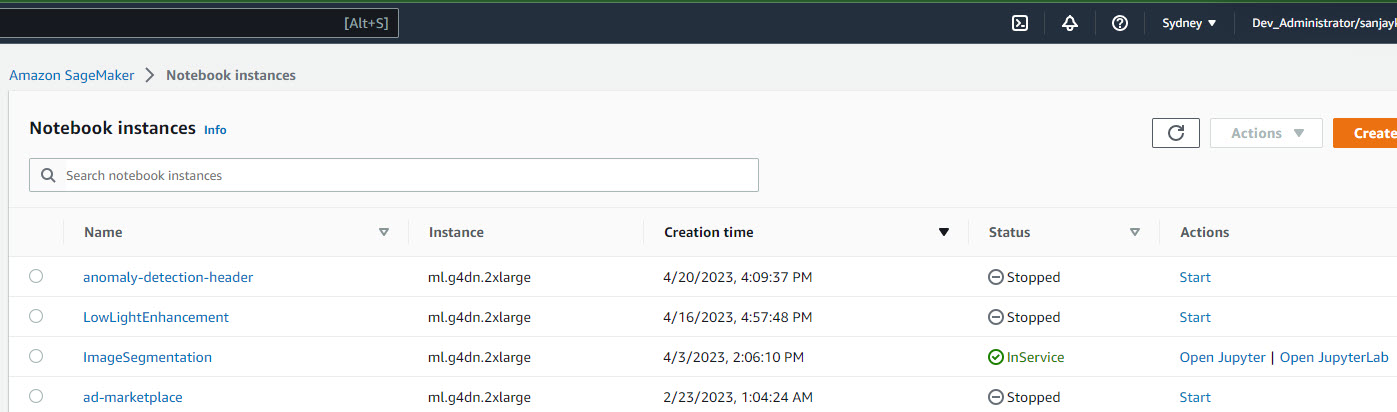
\includegraphics[width=420]{tool.jpg}
      \caption{Screenshot of Amazon Sagemaker tool.}
\end{figure}

\end{frame}
%----

%------------------------------------------------
\begin{frame}{Project Implementation - Algorithm}
    % Throughout your presentation, if you choose to use \section{} and \subsection{} commands, these will automatically be printed on this slide as an overview of your presentation
    \tableofcontents
%------------------------------------------------
%Hyperparameters tuning
%------------------------------------------------

 %Adding picture

  \begin{figure}
   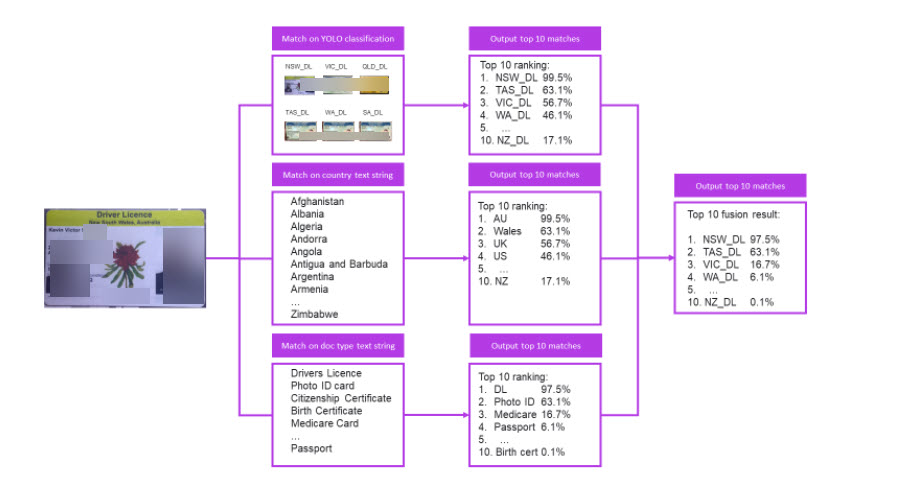
\includegraphics[width=340]{dia.jpg}
      \caption{Supplement text strings with YOLO image classification model for all supported ID documents}
\end{figure}

\end{frame}
%----

% Sanjay Issues Explanation in details
%------------------------------------------------
\begin{frame}{Results and Achievements}
    % Throughout your presentation, if you choose to use \section{} and \subsection{} commands, these will automatically be printed on this slide as an overview of your presentation
    \tableofcontents
%------------------------------------------------
%Hyperparameters tuning
%------------------------------------------------
    \begin{columns}[c] % The "c" option specifies centered vertical alignment while the "t" option is used for top vertical alignment

        \column{.45\textwidth} % Left column and width
        \textbf{Key Steps and Milestone}
        \begin{enumerate}
            \item SIFT Method for Document Match.
            \item APCER/BPCER Methods.
        
        \end{enumerate}

        \column{.5\textwidth} % Right column and width
         For Text OCR used APCER/ BPCER method for overall error rate classification and for image template used SIFT method.

    \end{columns}   \\
 %Adding picture

  \begin{figure}
   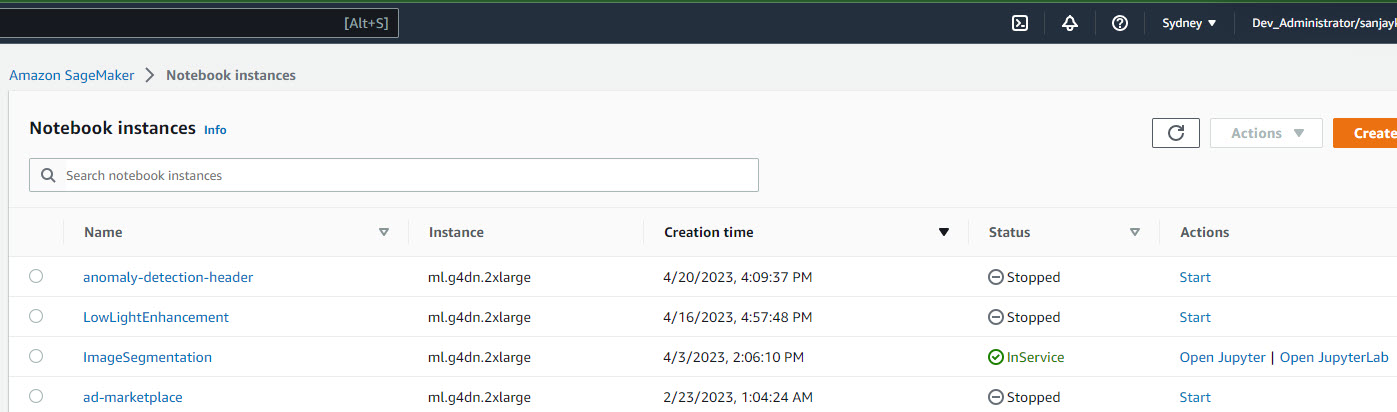
\includegraphics[width=420]{tool.jpg}
      \caption{Screenshot of Amazon Sagemaker tool.}
\end{figure}

\end{frame}
%----
% Findings and conclusion for the project
%------------------------------------------------
\begin{frame}{Conclusion}
    \tableofcontents
%------------------------------------------------
%Overview
%------------------------------------------------

    \begin{columns}[c] % The "c" option specifies centered vertical alignment while the "t" option is used for top vertical alignment

        \column{.45\textwidth} % Left column and width
        \textbf{The Process}
        \begin{enumerate}
            \item Overall, Designed, build, and documented process to improve the Text format check...
            \item Overall, Designed, build, and improve the Visual Feature check.. 
        \end{enumerate}

        \column{.5\textwidth} % Right column and width
         Ensured the task Text format/ Visual feature check was implemented as per the requirement along with it the team was able to find and validate and execute the code in the production system and were able to improve the OCR error by 10 percent in Visual Feature Check.

    \end{columns}   \\

\end{frame}
%------------------------------------------------



\end{document}